\actTitle{1.7 - Piecewise Define Functions and Analysis of Graphs}

\videoLink{Section 1.7}{https://www.youtube.com/playlist?list=PLYHZK3b8UFw0MGYUVN9Z4aYof_QgbFw7f}

\noindent \textbf{Topics:}  basic functions, even and odd functions, graphing piecewise functions, relative minima and maxima\\

\noindent \textbf{Student Learning Outcomes:}
\begin{enumerate}
\item Students will be able to determine whether a function is even, odd, or neither.
\item Students will be able to graph a piecewise function.
\item Students will be able to determine where a function is increasing, decreasing, or constant.
\item  Students will be able to locate relative minimum and relative maximum values of a function on a graph.
\end{enumerate}

\hrule 

\bigskip

\subsection{Even and Odd Functions} ~



\noindent
\fbox{
  \parbox{\dimexpr\linewidth}%
  {
    We call $f$ an \emph{even} function if the graph of $f$ is
    symmetric with respect to the $y$ axis. In that case, $f(-x)=f(x)$
    for every $x$ in the domain.
  }
}

\noindent
\fbox{
  \parbox{\dimexpr\linewidth}%
  {
    We call $f$ an \emph{odd} function if the graph of $f$ is
    symmetric with respect to the origin. In that case, $f(-x)=-f(x)$
    for every $x$ in the domain.
  }
}


\begin{enumerate}
\item Determine whether $f$ is even, odd, or neither. 
\begin{enumerate}
\item $f(x)=17x^3-12x^5$
  \vfill
\item $f(x)=x^3-5x^2$
  \vfill
\item $f(x)=|x|$ (This is the \emph{absolute value function}). %Sketch its graph below.
  \vfill
\end{enumerate}



\clearpage


\subsection{Piecewise-Defined Functions} ~

\noindent
\fbox{
  \parbox{\dimexpr\linewidth}%
  {

    \underline{Piecewise-Defined Functions.}  \\
    \noindent
    A \emph{piecewise function} is a function defined by multiple
    sub-functions with each sub-function applying to a certain
    interval of the main function's domain.
  }
}


\item Evaluate the function for the given values of $x$ and then graph the function.
\[
  f(x) =
  \begin{cases}
                                   -x-1 & \text{for $x<1$} \\
                                   -3 & \text{for $1 \leq x <2$} \\
  \sqrt{x-2} & \text{for $x \geq 2$}
  \end{cases}
\]

\begin{enumerate}
\item $f(-3)=$
  \vfill
\item $f(1)=$
  \vfill
\item $f(2)=$
  \vfill
\item $f(6)=$
  \vfill
\item Graph $f(x)$
\end{enumerate}


      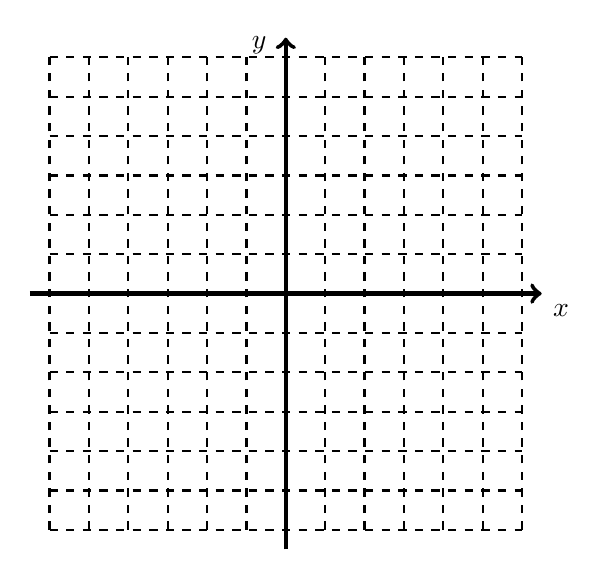
\begin{tikzpicture}[y=0.5cm, x=0.5cm,font=\sffamily]
        \begin{scope} %[shift={(0,8)}]
          %% ticks
          \draw[xstep = 1, ystep=1.0,black,dashed,thick] % very thin,opacity=0.85,
                 (-6.0,-6.0) grid ( 6.0, 6.0);
             %% axis
           \draw[ultra thick,->] (-6.5,0) -- coordinate (x axis mid) (6.5,0)
                node[anchor = north west] {$x$}; 
           \draw[ultra thick,->] (0,-6.5) -- coordinate (y axis mid) (0,6.5) 
                node[anchor = east,shift={(-0.2,-0.2)}]  {$y$};

           %\foreach \y in {-1,1,...,4} {
           %   \draw (1pt, \y) -- (-1pt, \y) node[yshift=-6,xshift=1,anchor=west] {$\y$};
           % }
           %\foreach \x in {-3,-2,-1,1,2,3} {
           %   \draw (\x,1pt) -- (\x,-1pt) node[yshift=-5,xshift=-1,anchor=east] {$\x$};
           % }

          \end{scope}
        \end{tikzpicture}



\clearpage



\item Graph the piecewise function.
\[
  f(x) =
  \begin{cases}
                                   x+3 & \text{for $x<-1$} \\
                                   x^2 & \text{for $-1 \leq x <2$} 
  \end{cases}
\]

      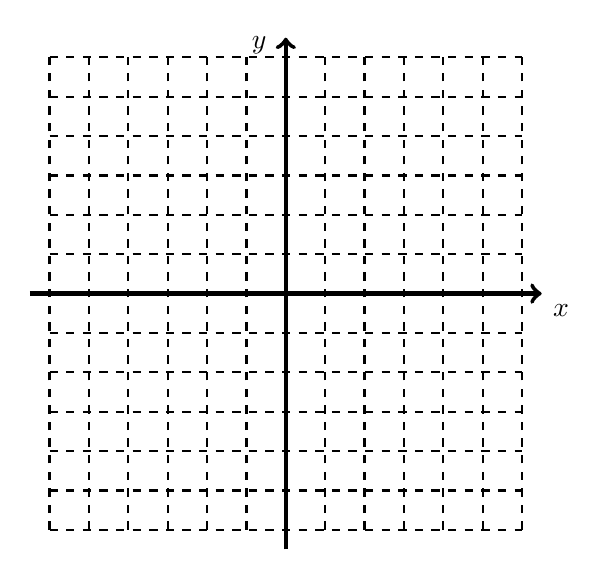
\begin{tikzpicture}[y=0.5cm, x=0.5cm,font=\sffamily]
        \begin{scope} %[shift={(0,8)}]
          %% ticks
          \draw[xstep = 1, ystep=1.0,black,dashed,thick] % very thin,opacity=0.85,
                 (-6.0,-6.0) grid ( 6.0, 6.0);
             %% axis
           \draw[ultra thick,->] (-6.5,0) -- coordinate (x axis mid) (6.5,0)
                node[anchor = north west] {$x$}; 
           \draw[ultra thick,->] (0,-6.5) -- coordinate (y axis mid) (0,6.5) 
                node[anchor = east,shift={(-0.2,-0.2)}]  {$y$};

           %\foreach \y in {-1,1,...,4} {
           %   \draw (1pt, \y) -- (-1pt, \y) node[yshift=-6,xshift=1,anchor=west] {$\y$};
           % }
           %\foreach \x in {-3,-2,-1,1,2,3} {
           %   \draw (\x,1pt) -- (\x,-1pt) node[yshift=-5,xshift=-1,anchor=east] {$\x$};
           % }

          \end{scope}
        \end{tikzpicture}

\subsection{Intervals of Increasing, Decreasing, and Constant Behavior}
When looking at functions on a graph, we read from left to right.
And when we talk about function values, we mean values on the $y$-axis.\\[.1in]

In this section, we will determine intervals on the $x$-axis where the
function values on the $y$-axis are increasing, decreasing, or
constant.

\item Determine where the following function is increasing, decreasing, or constant.

      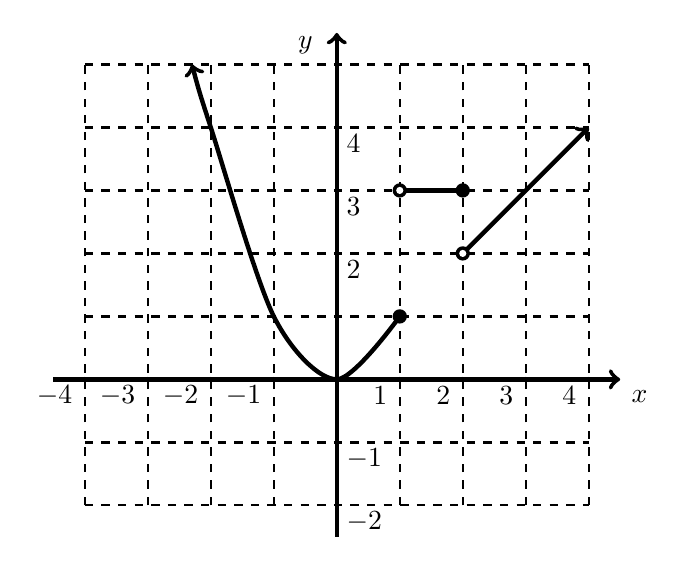
\begin{tikzpicture}[y=0.8cm, x=0.8cm,font=\sffamily]
        \begin{scope} %[shift={(0,8)}]
          %% ticks
          \draw[xstep = 1, ystep=1.0,black,dashed,thick] % very thin,opacity=0.85,
                 (-4.0,-2.0) grid ( 4.0, 5.0);
             %% axis
           \draw[ultra thick,->] (-4.5,0) -- coordinate (x axis mid) (4.5,0)
                node[anchor = north west] {$x$}; 
           \draw[ultra thick,->] (0,-2.5) -- coordinate (y axis mid) (0,5.5) 
                node[anchor = east,shift={(-0.2,-0.2)}]  {$y$};

           \foreach \y in {-2,-1,2,3,4} {
              \draw (1pt, \y) -- (-1pt, \y) node[yshift=-6,xshift=1,anchor=west] {$\y$};
            }
           \foreach \x in {-4,-3,-2,-1,1,2,3,4} {
              \draw (\x,1pt) -- (\x,-1pt) node[yshift=-5,xshift=-1,anchor=east] {$\x$};
            }
          \end{scope}

          \begin{scope}
            \draw[ultra thick,<-] plot [smooth] coordinates
                {(-2.3,5) (-2,4) (-1,1) (0,0) (1,1) };
            \fill[black] (1,1) circle [radius=0.6ex]; 

            \draw[black,ultra thick] (1,3) -- (2,3);
            \fill[black] (1,3) circle [radius=0.6ex]; % Draw an open dot on the 
            \fill[white] (1,3) circle [radius=0.3ex]; 
            \fill[black] (2,3) circle [radius=0.6ex]; % Draw an open dot on the 

            \draw[black,ultra thick,->] (2,2) -- (4,4);
            \fill[black] (2,2) circle [radius=0.6ex]; % Draw an open dot on the 
            \fill[white] (2,2) circle [radius=0.3ex]; 

          \end{scope}
        \end{tikzpicture}

\clearpage

\subsection{Relative Minimum and Relative Maximum Values}
Remember, when talking about function \textbf{values}, we mean
$y$-values.  So in this section we will determine the relative minimum
and maximum $y$-values of a function.

\item For the graph of $y=f(x)$ shown.

        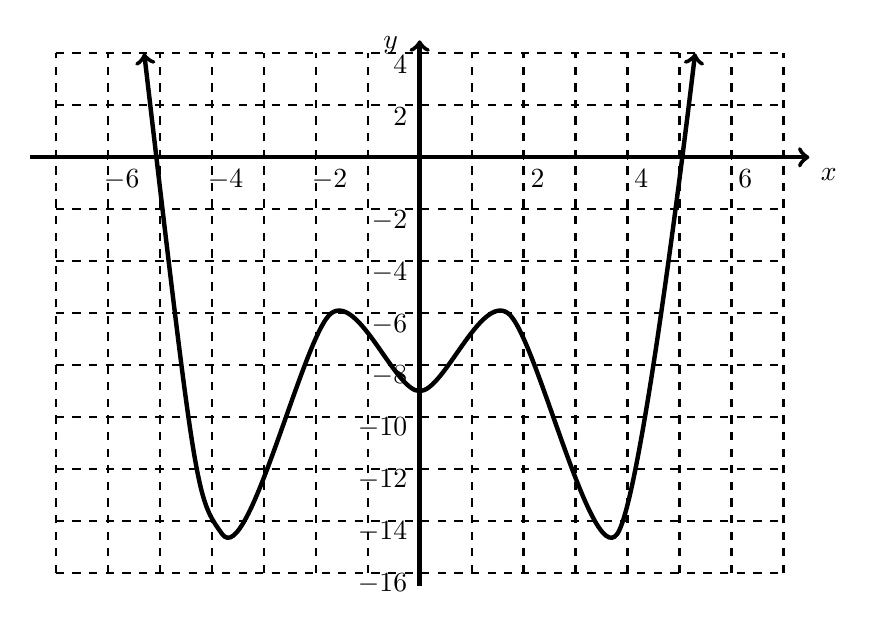
\begin{tikzpicture}[y=0.33cm, x=0.66cm,font=\sffamily]
          \begin{scope} %[shift={(0,8)}]
          %% ticks
          \draw[xstep = 1, ystep=2.0,black,dashed,thick] % very thin,opacity=0.85,
                 (-7.0,-16.0) grid ( 7.0, 4.0);
             %% axis
           \draw[ultra thick,->] (-7.5,0) -- coordinate (x axis mid) (7.5,0)
                node[anchor = north west] {$x$}; 
           \draw[ultra thick,->] (0,-16.5) -- coordinate (y axis mid) (0,4.5) 
                node[anchor = east,shift={(-0.2,-0.2)}]  {$y$};

           \foreach \y in {-16,-14,...,-2,2,4} {
              \draw (1pt, \y) -- (-1pt, \y) node[yshift=-4,xshift=0,anchor=east] {$\y$};
            }
           \foreach \x in {-6,-4,-2,2,4,6} {
              \draw (\x,1pt) -- (\x,-1pt) node[yshift=0,xshift=5,anchor=north] {$\x$};
            }
          \end{scope}

          \begin{scope}
            \draw[ultra thick,<->] plot [smooth] coordinates
            {(-5.3,4) (-3.8,-14.5) (-1.7,-6) (0,-9)
             (1.7,-6) (3.8,-14.5) (5.3,4) };
          \end{scope}
        \end{tikzpicture}

\begin{enumerate}
\item Determine the location and value of any relative maxima.\\[.3in]
\item Determine the location and value of any relative minima.
\end{enumerate}

\vfill
\end{enumerate}

\noindent \textbf{Student Learning Outcomes Check}

\begin{enumerate}
\item Can you determine whether a function is even, odd, or neither?
\item Can you graph a piecewise function?
\item Are you able to determine where a function is increasing, decreasing, or constant?
\item  Can you locate relative minimum and relative maximum values of a function on a graph?

\end{enumerate}

\noindent \textbf{If any of your answers were no, please ask about these topics in class.}


